\begin{frame}{Ambient Reflection - Mathematics}
  \begin{columns}
    \begin{column}{0.6\textwidth}
      \small
      \begin{mathbox}{Ambient Component Formula}
        \textbf{Simplest lighting component:}
        \begin{align*}
          I_{\text{ambient}} = \mathbf{k}_a \odot \mathbf{I}_a
        \end{align*}

        \begin{itemize}
          \item $\mathbf{k}_a$ = ambient reflection coefficient of the material
          \item $\mathbf{I}_a$ = intensity of ambient light in the scene
        \end{itemize}
        \only<2->{
          \vspace{0.3cm}
          \textbf{Key properties:}
          \begin{itemize}
            \item Independent of viewer position, light direction, or surface normal
            \item $\mathbf{I}_a$ is a constant for the scene or a combination of the light sources in the scene
          \end{itemize}
        }
      \end{mathbox}
    \end{column}
    \begin{column}{0.4\textwidth}
      \only<3->{
        \begin{figure}
          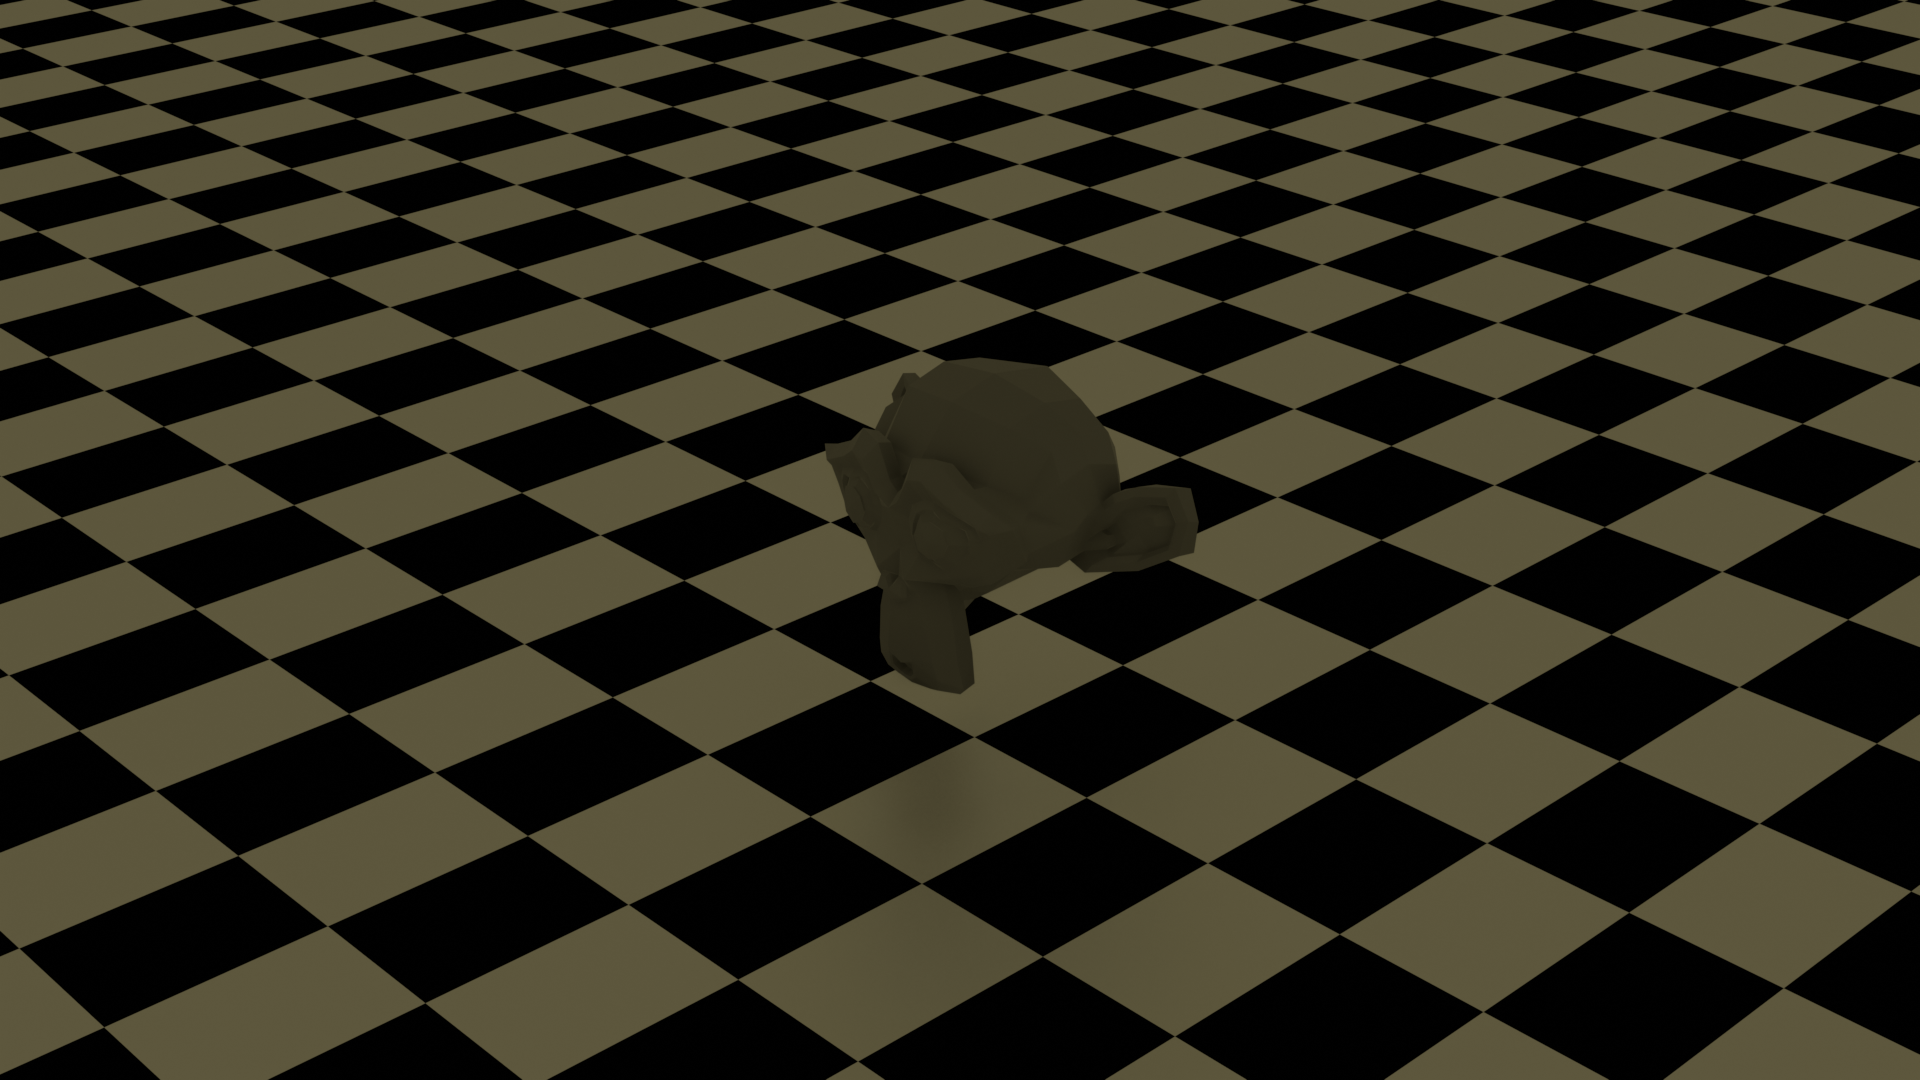
\includegraphics[width=\linewidth]{images/low_amb.png}
          \caption*{Low $\mathbf{k}_a$}
        \end{figure}
        \begin{figure}
          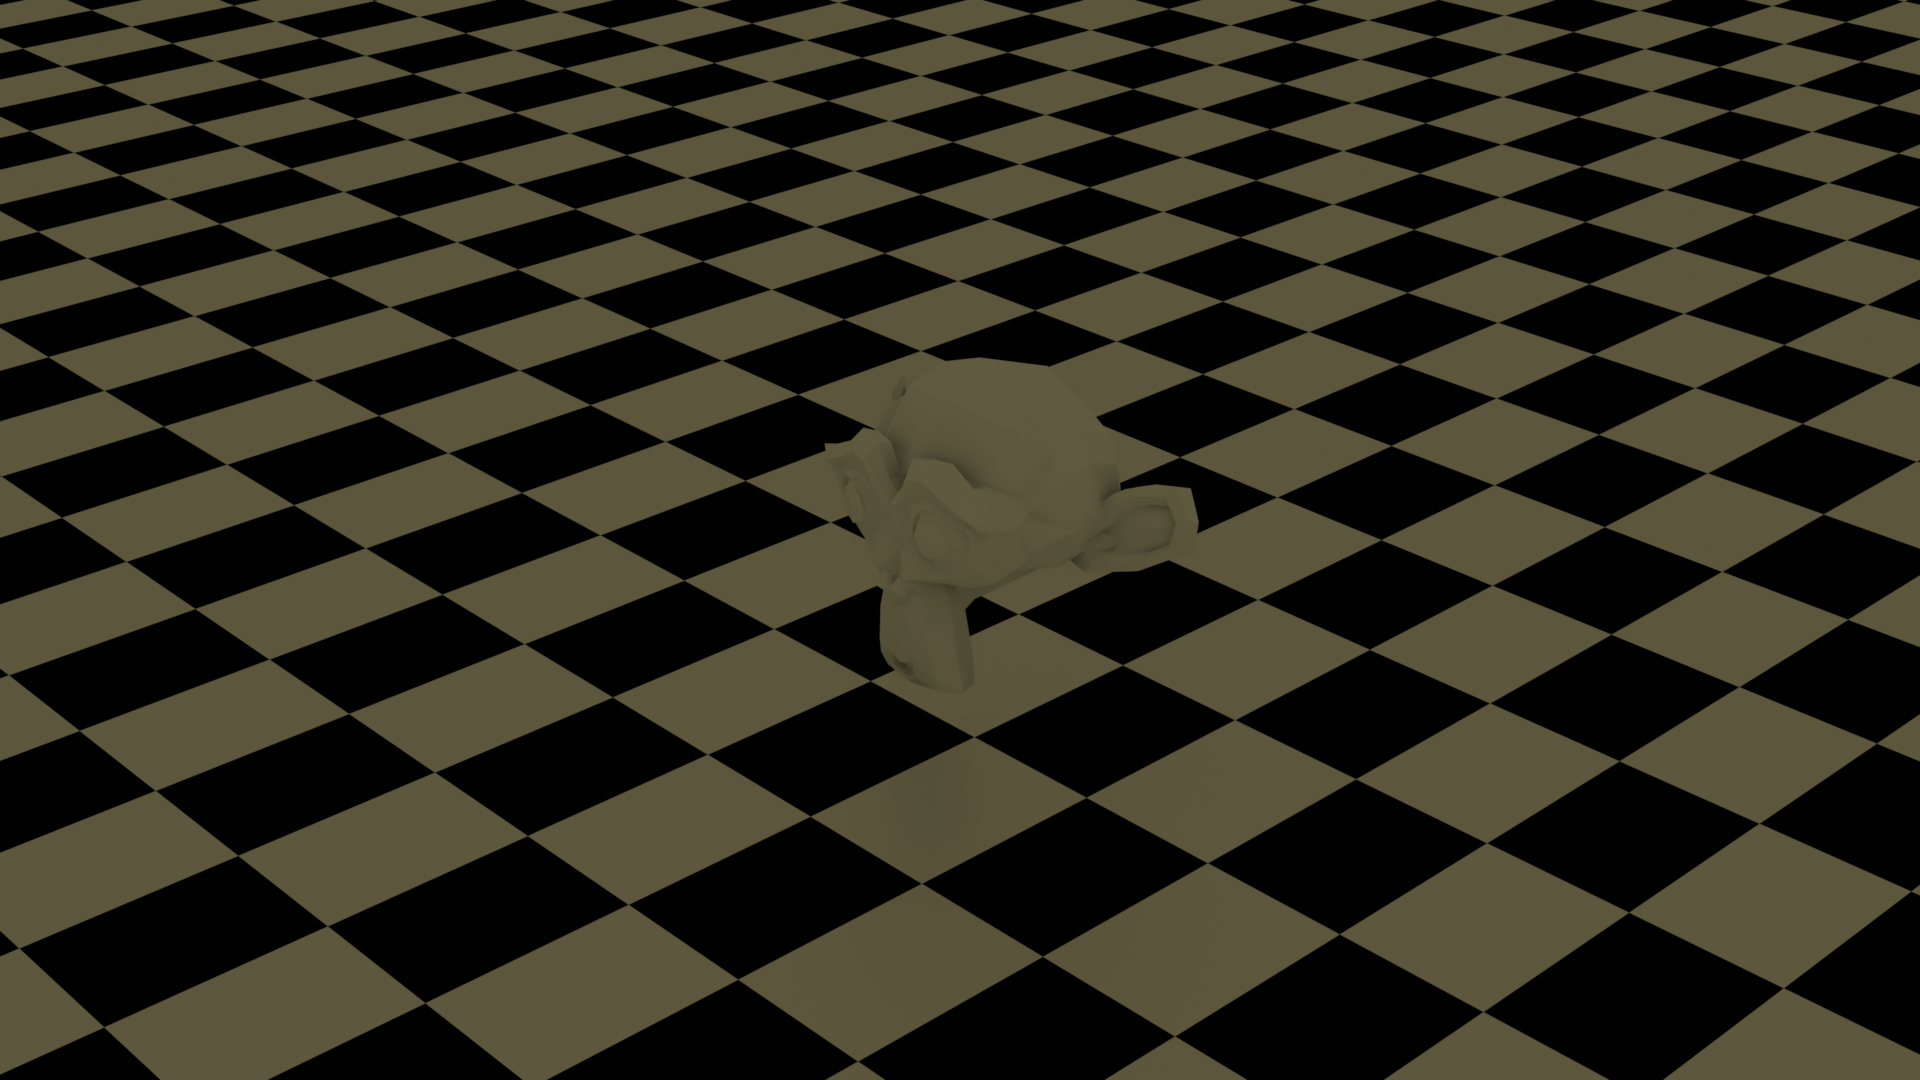
\includegraphics[width=\linewidth]{images/ambient.png}
          \caption*{High $\mathbf{k}_a$}
        \end{figure}
      }
    \end{column}
  \end{columns}
\end{frame}
